% !TeX spellcheck = en_US
\documentclass[]{article}

\title{RuleRank Ultimate Desktop Edition Manual 1.0}
\author{Piotr Jówko}

\usepackage{graphicx}
\usepackage{chngpage}
\graphicspath{ {./images/} }

\usepackage[english]{babel}
\usepackage{hyperref}

\hypersetup{
	pdffitwindow=true,
	bookmarksnumbered=true,
	bookmarksopen=true,
	colorlinks=true,
	pdfpagelayout=SinglePage,
	pdfpagemode=UseOutlines,
	pdfstartview=Fit,
	linkcolor=black,
	citecolor=black,
	anchorcolor=black,
	filecolor=black,
	menucolor=black,
	urlcolor=blue,
	pdftitle={},
	pdfauthor={},
	pdfkeywords={}
}

\begin{document}

% First Page start
\vspace*{0.5cm}
\begin{center}
	Pozna\'n University of Technology\\Faculty of Computing\\Institute of Computing Science
\end{center}
\vspace{2cm}
\begin{center}
	\hspace*{-0.4cm}\Large\bfseries\MakeUppercase{RuleRank Ultimate Desktop Edition User Manual 1.0}
	\par\vspace{0.1cm}
\end{center}
\vspace*{1.2cm}
\begin{center}
	\begin{Large}
		Author:
	\end{Large}
	\begin{Large}
		Piotr Jówko
	\end{Large}
\end{center}
\vspace{4cm}\begin{center}Poznań, \today\end{center}
\vspace{1.5cm}
% First Page end
\newpage

% !TeX spellcheck = en_US
\begin{Large}
	About RUDE application
\end{Large}
\newline

RuleRank Ultimate Desktop Edition (RUDE) is a JavaFX application with uses java Rough Sets library (jRS). Application supports Windows, Linux and Mac operating systems. It requires Java 10 to run.
\newline

It provides rich user interface to create own experiments concerning multicriteria ranking problems using Dominance-based Rough Set Approach and Variable Consistency Dominance-based Rough Set Approach.
\newline

First chapter describes RUDE installation process on a local computer. The rest of the document describes all features of this application.

\vfill\newpage

\tableofcontents
\newpage

% !TeX spellcheck = en_US
\section{Installation}\label{section:install}

Application supports Windows, Linux and Mac operating systems. It requires Java 10 JRE or JDK to be installed. The newest version of Java can be downloaded here:\\ \href{http://www.oracle.com/technetwork/java/javase/downloads/index.html}{http://www.oracle.com/technetwork/java/javase/downloads/index.html}


RUDE application doesn't require installation. You simply need to download archived application and extract it to some directory. You can download it from here:\\ \href{http://www.cs.put.poznan.pl/mszelag/Software/ruleRank/ruleRank.html}{http://www.cs.put.poznan.pl/mszelag/Software/ruleRank/ruleRank.html}\newline

\textbf{Archive content description:}
\begin{itemize}
	\item \textbf{data directory} - it contains configuration files, see \hyperref[section:data-config]{Data configuration}
	\item \textbf{workspace directory} - it is default directory for storing all files related to experiments. It also contains some example experiments with result files.
	\item \textbf{readme.txt} - it contains information about requirements and running application
	\item \textbf{RuleRank jar file} - it contains compiled sources for this application
	\item \textbf{run.* files} - files which will run application after double click. Run files were prepared for each supported operating system.
\end{itemize}

You can run application by double clicking on respective run file. It will open console/terminal and run UI application. In case of any problems with running RUDE, error logs will be displayed in console/terminal. If you encounter any errors, it is recommended to execute run file in cmd/powershell or terminal, instead of double clicking. It will not close console/terminal after application exit.


\vfill\newpage
% !TeX spellcheck = en_US
\section{Application overview}\label{section:overview}

In this chapter we will provide general overview of main application window.

\begin{figure*}[!ht] 
	\centering
	\makebox[\textwidth]{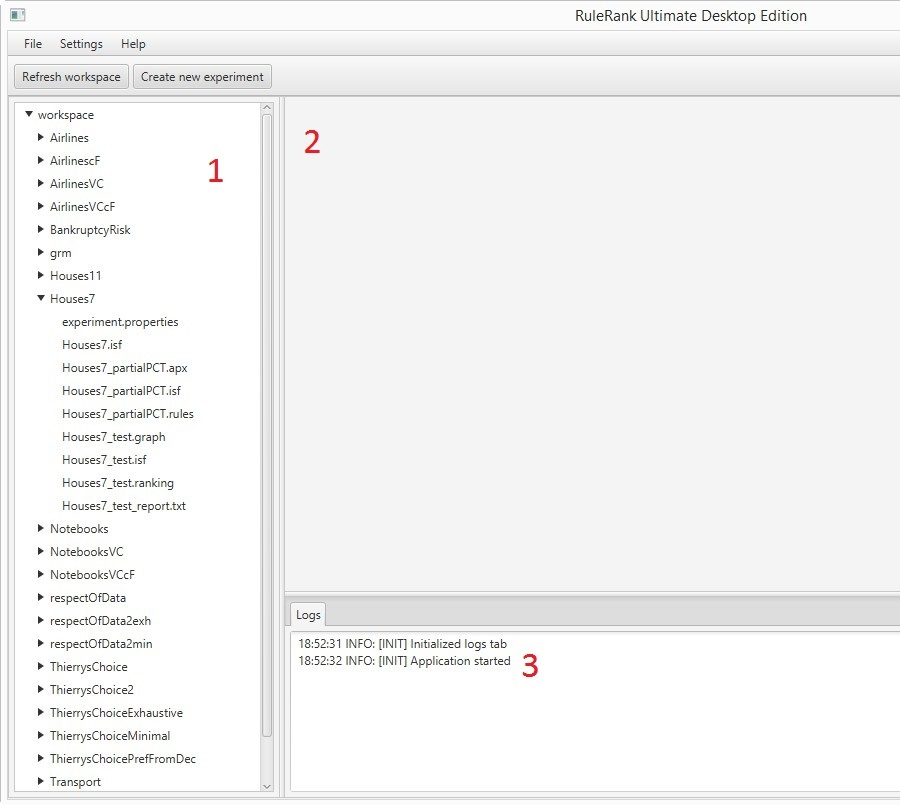
\includegraphics[width=.7\paperwidth]{overview}}
	\caption{Main window screen}
\end{figure*}

There are three main panels in RUDE application:
\begin{itemize}
	\item workspace(1) - it manages all files
	\item upper panel(2) - it displays most of the information. It can display multiple tabs like web browser. Most of the work will be done here.
	\item lower panel(3) - it contains logs and can display additional information for some upper tabs. It can display multiple tabs like web browser.
\end{itemize}

On top of main window you can find menu:
\begin{itemize}
	\item File - it currently enables to quit program
	\item Settings - it contains user settings for RUDE application
	\item Help - it contains About and Help modal dialogs.
\end{itemize}

Below menu you can find toolbar with actions, with will be described in \hyperref[section:workspace]{Workspace management section}.\\


\textbf{Logs tab:}\\
Logs tab display all logs from application. 
Currently there are three logs levels:
\begin{itemize}
	\item INFO - displays some useful information about performed actions
	\item WARN - indicates some misconfiguration or action aborting in certain conditions. It also indicates errors handled by application.
	\item ERROR - displays errors not handled properly by application
\end{itemize}

Logs can be copied by selecting text and pressing Ctrl + C. All logs can be clear by right clicking on logs panel and choosing "Clear logs" option.

\vfill\newpage
% !TeX spellcheck = en_US
\section{User settings}\label{section:user-settings}

TODO

\vfill\newpage
% !TeX spellcheck = en_US
\section{Workspace management}\label{section:workspace}

In this chapter we will describe all features of workspace panel.

Workspace panel displays all files and directories(items) from workspace directory. Items are displayed in hierarchical structure representing hierarchy in file system. It also allows to do some basic file management. Thanks to this features, user doesn't have to exit program when he want to manage files. Path to workspace can be configured in user settings. See \hyperref[section:user-settings]{User settings section}.

\begin{figure*}[!ht] 
	\centering
	\makebox[\textwidth]{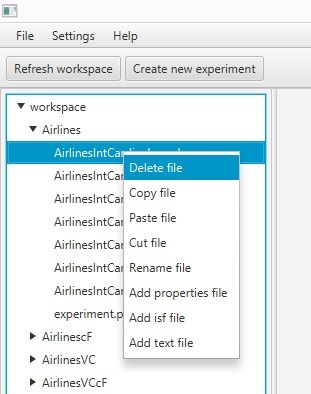
\includegraphics[width=.35\paperwidth]{workspace}}
	\caption{Application workspace from left panel}
\end{figure*}

Most of workspace functionality is provided by context menu, with is accessible by right clicking on workspace item(file or directory). If directory contains files or other directories, it will have arrow on left side indicating, that item can be expanded/hided. Buttons on toolbar are also used for workspace management. They contain actions with are not related with specific item. File can be opened by double clicking on it.

Some actions support keyboard shortcuts. To perform action by shortcut, you have to select item and press specific combination of keyboard buttons described below:
\begin{itemize}
	\item \textbf{Ctrl + C} - copies selected file to user clipboard. Copying directories is not supported yet.
	\item \textbf{Ctrl + V} - paste file to selected directory. If file was selected, file from clipboard will be copied to same directory as selected file.
	\item \textbf{Ctrl + X} - cuts file to user clipboard. If you paste file, old file will be removed.
	\item \textbf{Ctrl + R} - open dialog to rename file.
\end{itemize}


Toolbar currently supports two actions:

\begin{itemize}
	\item \textbf{Refresh workspace} - it refresh first level of workspace tree. If some directories were expanded deeper, they will be hided.
	\item \textbf{Create new experiment} - it allows to create new experiment with example isf table and experiment properties file. It will open dialog with shows workspace. You should create new directory there or choose existing directory.
\end{itemize}


It is recommended to create separate directory for each experiment. Learning or test data table(isf files) can be stored in commonly shared folders. Each directory should contain only one experiment properties file. This file is needed for other files to extract information about experiment. Also it is recommended to store results files in same directory as experiment properties file.\\

Below is supported file type list:
\begin{itemize}
	\item \textbf{.properties} - contains experiment properties with is used to configure experiment. See \hyperref[section:properties]{Experiment properties section}.
	\item \textbf{.isf} - contains tabular data with can be editable or read only depending on data type. Here you can configure learning or test data for experiment. You can also view partial pairwise comparison table generated by experiment.
	See \hyperref[section:isf-table]{Isf table edition section} and  \hyperref[sub:pct-isf]{Partial PCT section}.
	\item \textbf{.apx} - contains some information about experiment in text format.
	See \hyperref[sub:pct-apx]{Partial PCT section}.
	\item \textbf{.rules} - contains generated rules and rules statistics.
	See \hyperref[section:rules]{Rules section}.
	\item \textbf{.graph} - contains preference graph visualization.
	See \hyperref[section:graph]{Graph visualization section}.
	\item \textbf{.ranking} - contains result ranking for experiment.
	See \hyperref[section:ranking]{Ranking window section}.
	\item \textbf{.txt} - it can be used to store some notes or to show experiment report
\end{itemize}

All other file types are not supported. Not supported files are treated as non editable text files.

\vfill\newpage
% !TeX spellcheck = en_US
\section{Isf table edition}\label{section:isf-table}

TODO

\vfill\newpage
% !TeX spellcheck = en_US
\section{Experiment properties}\label{section:properties}

In this chapter we will describe experiment configuration. To edit experiment configuration, you have to double click on .properties file in workspace tree.\\

Four windows are used to configure experiment:
\begin{itemize}
	\item \textbf{Properties form} - this is tab with opens after double click on properties file. It allows to edit experiment configuration.
	\item \textbf{Default properties form} - it is special case of properties form, where default properties for all experiments all configured.
	\item \textbf{Ranking dialog} - this modal dialog supports user friendly object ranking edition.
	\item \textbf{Pairs dialog} - this modal dialog supports user friendly comparison pairs edition
\end{itemize}

All windows are described in sections below.

\subsection{Properties form}\label{sub:properties-form}

With default user settings, properties form will be opened with hidden sections of properties. This sections can be expanded by clicking on them. You can change this settings in User settings dialog. See \hyperref[section:user-settings]{User settings section}.

\begin{figure*}[!ht] 
	\centering
	\makebox[\textwidth]{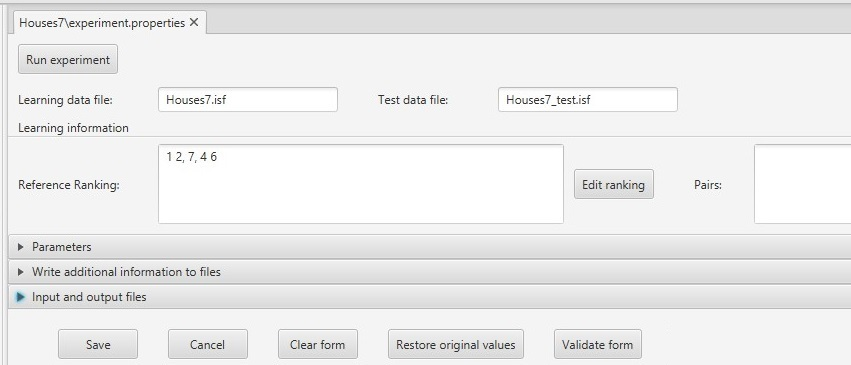
\includegraphics[width=.65\paperwidth]{properties}}
	\caption{Properties form with default settings}
\end{figure*}

On top of the form, there is learning and test data table path. Learning data file is required field. If you hover on field with default user settings, tooltip with help will be displayed. You should also configure ranking or pairs before running experiment.

On bottom of the screen following actions can be performed:
\begin{itemize}
	\item \textbf{Clear form} - clears all fields.
	\item \textbf{Restore original values} - restores values for all fields, as they were loaded from file again.
	\item \textbf{Validate form} - performs validation on form for all fields, including default ones. When running experiment, empty values from properties are replaced with default ones. It can discover issues with configuration, when values from form and default properties are not correctly set. If you find such issue, you should change settings in your experiment or in default properties.
\end{itemize}

Below, we describe meaning of all parameters.
\begin{itemize}
	\item \textbf{Learning data file} - absolute or relative path to learning isf file. Directories must be separated by $\backslash$ character.
	\item \textbf{Test data file} - absolute or relative path to test isf file. Directories must be separated by $\backslash$ character. If not configured, it is assumed, that learning file is also test file.
	\item \textbf{Reference ranking} - initial ranking of objects in experiment.
	\item \textbf{Pairs} - pairs of object in outranking (S) or non-outranking (Sc) relation.
	\item \textbf{Type of family criteria} - can be consistent or any.
	\item \textbf{Type of rules} - can be certain of possible.
	\item \textbf{Considered set of rules} - if exhaustive, virtual exhaustive set of rules will be considered, if minimal, explicit minimal set of rules induced by VC-DomLEM algorithm will be considered.
	\item \textbf{Consistency measure} - measure used to calculate lower approximations of S and Sc relations.
	\item \textbf{Consistency measure threshold} - floating point number from [0,1] for epsilon, epsilon* and rough membership, or greater or equal than 0 for epsilon'.
	\item \textbf{Ranking procedure} - method used for calculating ranking from preference graph.
	\item \textbf{Dominance} - dominance relation used to calculate approximations of S and Sc relations in PCT.
	\item \textbf{Dominance for pairs of ordinal values} - indicator of the considered definition of dominance pairs of ordinal values in PCT.
	\item \textbf{Satisfaction degrees in preference graph} - weights in the preference graph. Can be fuzzy (from [0,1]) or crisp (0 or 1). Fuzzy satisfaction degree cannot be used with DRSA with exhaustive set of possible rules and rough membership.
	\item \textbf{Fuzzy satisfaction degree calculation method} - method for calculating fuzzy satisfaction degree in preference graph. Can be maximum of credibility over covering rules (max credibility) or maximum product of credibility and coverage factor over covering rules.
	\item \textbf{Negative examples treatment for VCDRSA} - sets strategy for covering negative examples by rules in VC-DRSA.
	\item \textbf{Rule conditions selection method in VCDomLEM} - strategy of rule conditions selection, either base (it can employ only elementary conditions built using evaluations of a single pair of objects) or mix (denotes that each rule can employ elementary conditions built using evaluations of different pairs of objects).
	\item \textbf{Optimize rule consistency in VCDomLEMWrt} - set of pairs of objects with respect to which value of rule consistency measure optimized in VC-DomLEM algorithm is calculated. Can be lower (or upper) approximation of the preference relation for which a certain (or possible, respectively) rule is generated or entire preference relation (for certain rules only) – either approximation or set.
	\item \textbf{Allow empty rules in VCDomLEM} - if true, rules with empty condition part can be generated if they have good consistency.
	\item \textbf{Use edge regions in VCDomLEM} - if true, only pairs of objects from EDGE region will be used to create rules condition.
	\item \textbf{Write domination information} - if true, sections [P-dominating sets] and [P-dominated sets] will be saved to .apx file.
	\item \textbf{Write rule statistics} - if true, rule statistics will be saved in .rule file.
	\item \textbf{Write learning positive examples} - if true, learning positive examples will be written to .rules file.
	\item \textbf{Precision} - denotes precision of floating point numbers when saving files. -1 disables rounding.
	\item \textbf{PCT file} - absolute or relative path on with isf file for Partial Pairwise Comparison Table will be saved. Directories must be separated by $\backslash$ character. If not given, name of the file will be set using learning data file name.
	\item \textbf{PCT Apx file} - absolute or relative path to .apx file, where approximations from PCT table will be saved. Directories must be separated by $\backslash$ character. If not given, name of the file will be set using learning data file name.
	\item \textbf{PCT rules file} - absolute or relative path on with rules will be saved. Directories must be separated by $\backslash$ character. If not given, name of the file will be set using learning data file name.
	\item \textbf{Preference graph file} - absolute or relative path on with graph will be saved. Directories must be separated by $\backslash$ character. If not given, name of the file will be set using test data file name.
	\item \textbf{Ranking file} - absolute or relative path on with ranking file will be saved. Directories must be separated by $\backslash$ character. If not given, name of the file will be set using test data file name.
\end{itemize}

\subsection{Default properties}\label{sub:properties-default}

When performing experiment, all properties must be set. So if user leave empty fields, they must be replaced with some default values. RUDE application have configurable default properties, with should be located in main workspace directory with file name: default.properties. You can edit this file freely, but it is recommended to fill all fields from parameters and write additional information sections.

\begin{figure*}[!ht] 
	\centering
	\makebox[\textwidth]{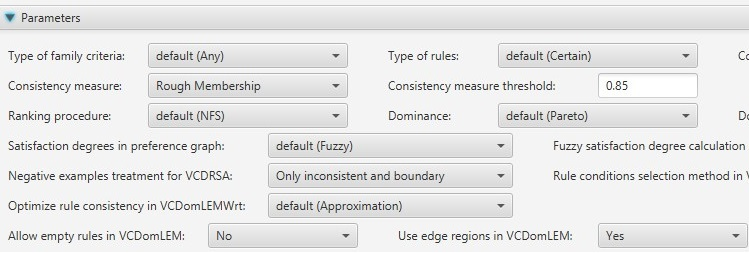
\includegraphics[width=.7\paperwidth]{properties-expanded}}
	\caption{Properties with default values set from default.properties file}
\end{figure*}

Default properties are loaded on each properties form. They are displayed to user in form: default (default value) for ComboBox fields, and as gray placeholder in other fields if they are empty. If you configure field in own experiment, value from your configuration will replace default one when performing experiment. All properties with are used in experiment are displayed in logs before experiment run.


\subsection{Ranking configuration}\label{sub:properties-ranking}

Ranking field represents initial ranking of objects in experiment. It can be edited by clicking on ''Edit ranking'' button.

Ranking can be configured manually in big text field, but it is not recommended and disabled by default. See \hyperref[section:user-settings]{User settings section}. Objects on left list are sorted by object ID.

\begin{figure*}[!ht] 
	\centering
	\makebox[\textwidth]{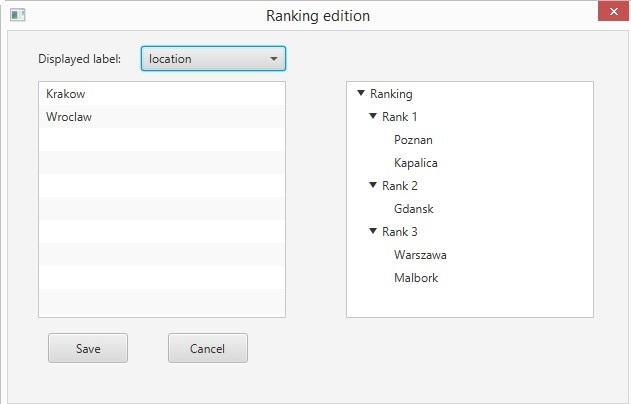
\includegraphics[width=.6\paperwidth]{properties-ranking}}
	\caption{Ranking edition modal dialog}
\end{figure*}

By default, objects ID (number of object) is displayed. If you created description attribute, it can be used as label for objects. You can change this in ''Displayed label'' field.

You can drag and drop objects from left list to right tree. If you place object on empty cell, new rank position will be created automatically. If you drag object to rank or element in rank, dragged object will be added to existing rank.

On right tree, you can perform two actions, with can be also invoked on selected item by context menu or keyboard shortcut:
\begin{itemize}
	\item \textbf{Remove selected (Delete)} - removes selected object from ranking. Removed object will return to list on the left. If rank was selected, all objects from rank will be removed to.
	\item \textbf{Add Rank below (A)} - adds new rank position below selected position.
\end{itemize}


\subsection{Pairs configuration}\label{sub:properties-pairs}

Pairs field represents comparison pairs of object in Pairwise Comparison Table. They can be edited by clicking on ''Edit pairs'' button.

Pairs can be configured manually in big text field, but it is not recommended and disabled by default. See \hyperref[section:user-settings]{User settings section}.

\begin{figure*}[!ht] 
	\centering
	\makebox[\textwidth]{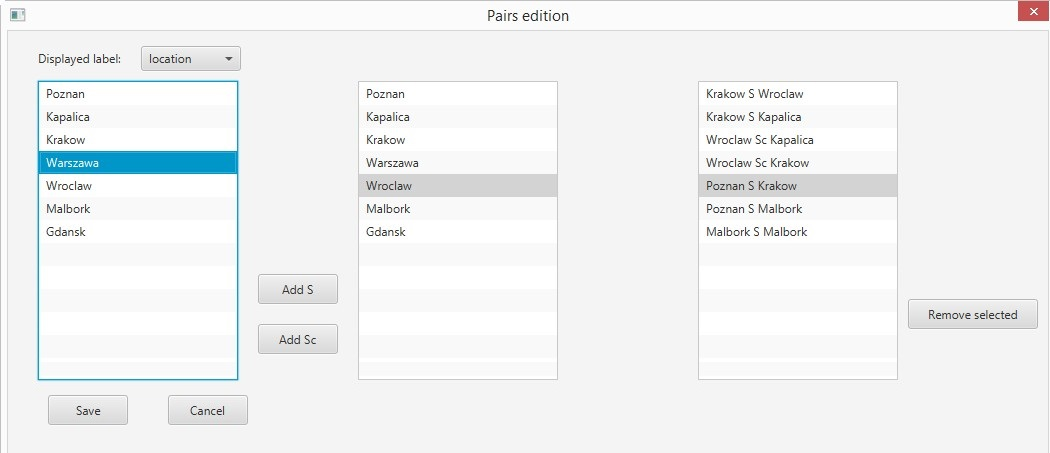
\includegraphics[width=.8\paperwidth]{properties-pairs}}
	\caption{Pairs edition modal dialog}
\end{figure*}

By default, objects ID (number of object) is displayed. If you created description attribute, it can be used as label for objects. You can change this in ''Displayed label'' field. 

First and second list contains all objects from experiment. Third list contains compared pairs of this objects with relation S (outranking) or Sc (non-outranking).

Three actions are available for this screen. Each can be invoked by pressing button, choosing option from context menu or by keyboard shortcut. First two actions are for first two lists, third is for pairs lists:
\begin{itemize}
	\item \textbf{Add S (S)} - adds selected pair of objects from first and second list to pairs lists. Objects are added in outranking relation.
	\item \textbf{Add Sc (C))} - adds selected pair of objects from first and second list to pairs lists. Objects are added in non-outranking relation.
	\item \textbf{Remove selected (Delete)} - removes selected pair from third list.
\end{itemize}



\vfill\newpage
% !TeX spellcheck = en_US
\section{Running experiment}\label{section:experiment-running}

In this chapter we will provide instructions for running experiment.

Before running experiment, learning data file (test data file is optional) should be created See \hyperref[section:isf-table]{Isf edition section}. It is recommended to fill all fields in active attributes. Condition attributes with empty values cannot be used in experiment, so experiment doesn't start with such values.

Also experiment properties should be configured. See \hyperref[section:properties]{Properties section}. All fields in properties should be set, either explicitly or by default values.

Experiment can be run from properties form. To do this, press ''Run Experiment'' button on top of properties form. After this isf table and experiment properties will be validated. If RUDE finds any misconfiguration error, it will display it on modal window and experiment doesn't start. If you provided multiple information sources (ranking, pairs or decision attribute), you will be asked to choose one of them.

\begin{figure*}[!ht] 
	\centering
	\makebox[\textwidth]{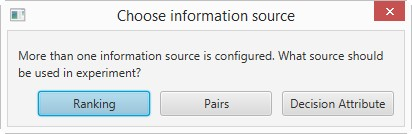
\includegraphics[width=.4\paperwidth]{raw/experiment-run-source}}
	\caption{Choose information source dialog}
\end{figure*}

Before experiment start, all properties will be logged (chosen properties and default ones for empty fields). When experiment finishes, all result files will be saved. In case of any errors, logs will be written to logs tab. Workspace tree will be automatically refreshed. If file names were not configured, they names will be calculated basing on learning and test data file name. The suffix partialPCT in some files is used to indicate that we deal with a “partial” PCT.

\vfill\newpage
% !TeX spellcheck = en_US
\section{Partial Pairwise Comparison Table}\label{section:pct}

In this section we will describe generated .isf and .apx file for Partial Pairwise Comparison Table. You can open this files by double clicking on them in workspace tree.

\subsection{Isf file}\label{sub:pct-isf}

This isf file is read only. Each row represents comparison of pair of examples. Each column represents attribute(criteria) on with comparison was performed.

\begin{figure*}[!ht] 
	\centering
	\makebox[\textwidth]{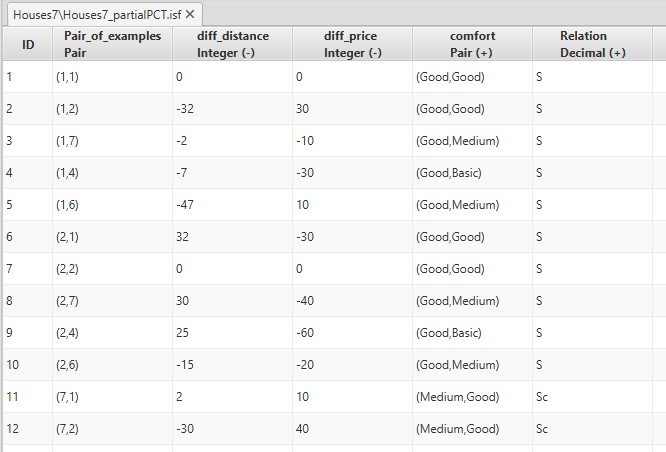
\includegraphics[width=.6\paperwidth]{raw/pct-isf}}
	\caption{Read only Partial Pairwise Comparison Table from Houses7}
\end{figure*}

In table header, field types and cost/gain criterion is displayed. If you hover over column header, additional information can be displayed. Columns can be ordered and sorted, but it will not be saved to file, because it is read only. You can also export selected rows to CSV format. You can do this by selecting rows and choosing "Copy selected rows" option from context menu.

\subsection{Apx file}\label{sub:pct-apx}

In this file additional information is saved in text format. User interface for this file is not created yet. It contains domination cons(P-dominating sets, P-dominated sets), approximations, decision classes and some metrics, like accuracy or quality of sorting.

\vfill\newpage
% !TeX spellcheck = en_US
\section{Rules}\label{section:rules}

In this section rules and rule statistic window is described. Rules and statistics are stored in .rules file. You can open this file by double clicking on it in workspace tree.

In some cases, rules can't be generated. In such case .no-rules file will be saved instead of rules file. Rules are generated from Pairwise Comparison Table.

\subsection{Rules window}\label{sub:rules}

\begin{figure*}[!ht] 
	\centering
	\makebox[\textwidth]{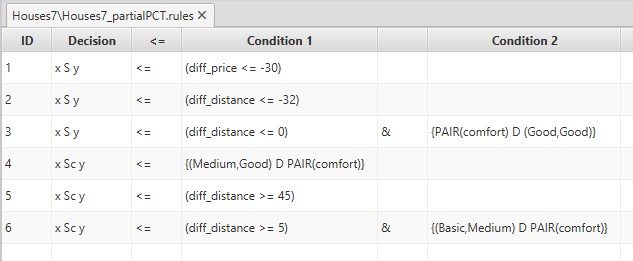
\includegraphics[width=.7\paperwidth]{raw/rules}}
	\caption{Rules tab from Houses7}
\end{figure*}

In this window all saved rules are displayed. Each rule consists of a conjunction of elementary conditions and a decision. Decision is always displayed on the left side. Each rule can have many conditions. Also, number of conditions in rules can vary for each rule. Values in columns can be sorted.\\

You can also export selected rules(rows) to CSV format. You can do this by selecting rows and choosing "Copy selected rows" option from context menu.\\

If you click on the rule, rule statistic tab will be displayed below. It displays additional information about rule and rule statistics.

\subsection{Rule statistics window}\label{sub:rule-stat}

In this tab rules statistics are displayed with some additional information about rule.
Rules can be of certain or possible type. Indexes provided in statistics represents position of pair in PCT file.\\\\

Some most important statistics are:
\begin{itemize}
	\item \textbf{Support} - number of pairs that supports this rule. Pair support rule if they belong to suggested relation and satisfies all elementary conditions.
	\item \textbf{Strength} - support / number of pairs.
	\item \textbf{Confidence} - also called certainty factor, defined as support / number of pairs of objects that satisfy all elementary conditions of rule.
	\item \textbf{Coverage factor} - support / number of pairs that belong to relation suggested by rule.
\end{itemize}

\begin{figure*}[!ht] 
	\centering
	\makebox[\textwidth]{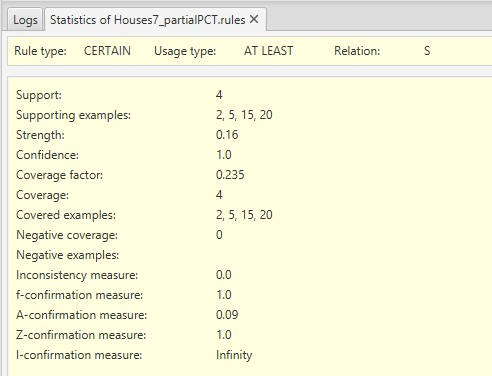
\includegraphics[width=.5\paperwidth]{raw/rules-stat}}
	\caption{Rules statistic tab from Houses7}
\end{figure*}

\vfill\newpage
% !TeX spellcheck = en_US
\section{Graph visualization}\label{section:graph}

In this section graph visualization window is described. Graph data is stored in .graph file. 
You can open this file by double clicking on it in workspace tree.

Preference graph is created from induced rules. Vertices of graph represents objects from isf table. 
Arcs represents outranking $S$ or non-outranking $S^{c}$ relations between objects. 
If arc is present between x and y vertices, it means that pair of x and y object is covered by a decision rule with suggest assignment to relation $S$ or $S^{c}$ relation. 
Arcs can be also weighted, where weight represents satisfaction degrees in preference relations.
Rule confidence is used for arc weight. 
If arc is covered by multiple rules, arc weight is aggregated, for example by taking maximum confidence.

\begin{figure*}[!ht] 
	\centering
	\makebox[\textwidth]{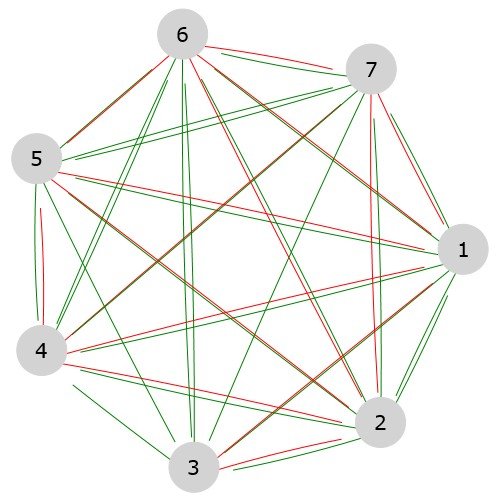
\includegraphics[width=.5\paperwidth]{raw/graph}}
	\caption{Graph visualization for Houses7}
\end{figure*}

Between each pair of vertices, up to four relations can be present:
\begin{itemize}
	\item $x S y$
	\item $x S^{c} y$
	\item $y S x$
	\item $y S^{c} y$
\end{itemize}

Relation type is marked with line color. Green is for outranking relation $S$ and red for non-outranking relation $S^{c}$. So relation $x S y$ will be drawn as green line between this two vertices.

All arcs are directed. Direction of arc is marked with line end. Lines ends before target vertex. So $x S y$ relation will be drawn as line from $x$ vertex to $y$ vertex with line ending slightly before $y$.

To improve arcs visibility, only up to two arcs are drawn between vertices. If verticles contain relations: $x S y$, $x S^{c} y$ - they will be replaced with one line with gray color. 
Same reduction is made for $y S x$, $y S^{c} x$.

You can navigate on graph by using scrollbars, zoom in and zoom out by mouse wheel. You can also drag vertices to change their position. If you click on vertex, it will be selected and summary for arcs will be displayed in tab below. All arcs weights can be displayed there (if they exists) in square brackets.

\begin{figure*}[!ht] 
	\centering
	\makebox[\textwidth]{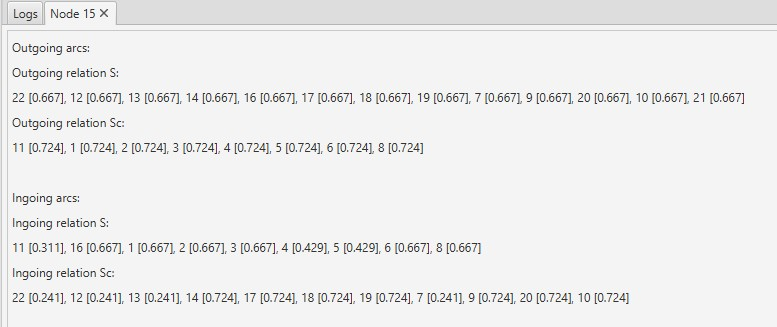
\includegraphics[width=.7\paperwidth]{raw/graph-arcs}}
	\caption{Vertex arcs for NotebooksVCcF with weights}
\end{figure*}


\vfill\newpage
% !TeX spellcheck = en_US
\section{Ranking window}\label{section:ranking}

TODO

\vfill\newpage
% !TeX spellcheck = en_US
\section{Minor features}\label{section:minor-features}

TODO


\subsection{Help window}\label{sub:minor-help}

TODO


\subsection{Text file edition}\label{sub:minor-txt}

TODO


\subsection{Unknown file types handling}\label{sub:minor-unknown}

TODO

\vfill\newpage
% !TeX spellcheck = en_US
\section{Data configuration directory}\label{section:data-config}

TODO


\subsection{Custom language support}\label{sub:config-labels}

TODO

\vfill\newpage

\end{document}
